\documentclass[border=8pt]{standalone}
\usepackage{tikz}
\usetikzlibrary{arrows.meta,positioning,calc,fit}
\begin{document}
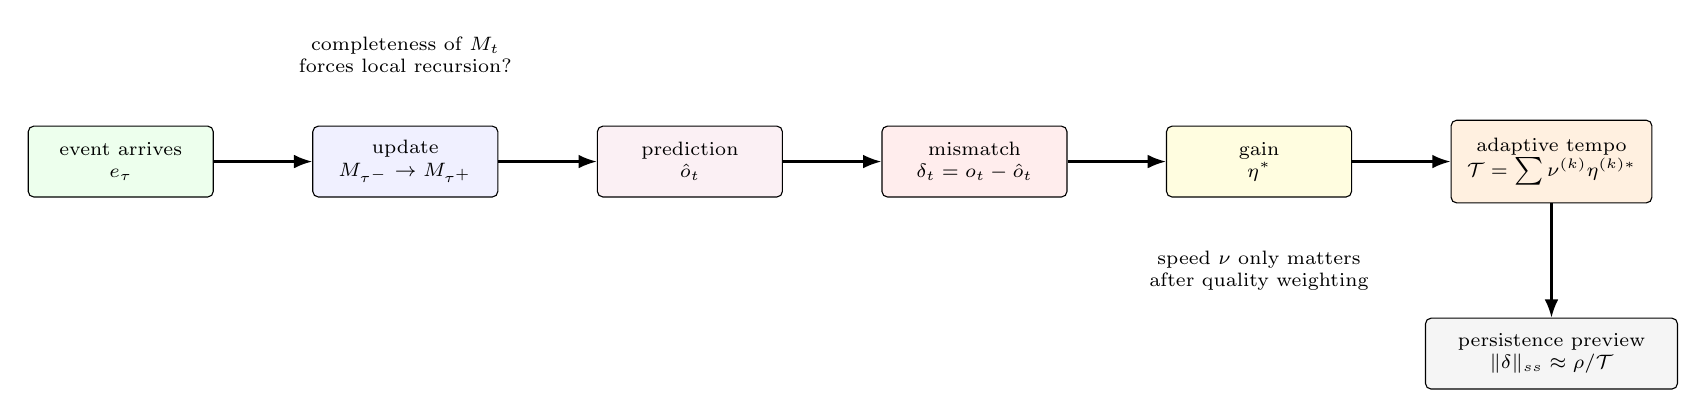
\begin{tikzpicture}[
  box/.style={draw, rounded corners=2pt, align=center, minimum width=2.35cm, minimum height=0.9cm, font=\scriptsize},
  capacitybox/.style={draw, rounded corners=2pt, align=center, minimum width=2.55cm, minimum height=1.05cm, font=\scriptsize, fill=orange!12},
  arr/.style={-Latex, thick},
  note/.style={align=center, font=\scriptsize}
]

\node[box, fill=green!7] (event) {event arrives\\$e_\tau$};
\node[box, fill=blue!6, right=1.25cm of event] (update) {update\\$M_{\tau^-}\to M_{\tau^+}$};
\node[box, fill=purple!6, right=1.25cm of update] (pred) {prediction\\$\hat o_t$};
\node[box, fill=red!7, right=1.25cm of pred] (mis) {mismatch\\$\delta_t=o_t-\hat o_t$};
\node[box, fill=yellow!12, right=1.25cm of mis] (gain) {gain\\$\eta^\ast$};
\node[capacitybox, right=1.25cm of gain] (tempo) {adaptive tempo\\$\mathcal T=\sum\nu^{(k)}\eta^{(k)\ast}$};

\draw[arr] (event) -- (update);
\draw[arr] (update) -- (pred);
\draw[arr] (pred) -- (mis);
\draw[arr] (mis) -- (gain);
\draw[arr] (gain) -- (tempo);

\node[box, fill=gray!8, below=1.45cm of tempo, minimum width=3.2cm] (persist) {persistence preview\\$\|\delta\|_{ss}\approx \rho/\mathcal T$};
\draw[arr] (tempo) -- (persist);

\node[note, above=0.55cm of update] {completeness of $M_t$\\forces local recursion?};
\node[note, below=0.55cm of gain] {speed $\nu$ only matters\\after quality weighting};

\end{tikzpicture}
\end{document}
